\documentclass{article}
    \usepackage[nonatbib]{nips_2016}
    
    \usepackage[breaklinks=true,letterpaper=true,colorlinks,citecolor=black,bookmarks=false]{hyperref}
    
    \usepackage{amsthm}
    \usepackage{amsmath,amssymb}
    \usepackage{enumitem}
    
    \usepackage[sort&compress,numbers]{natbib}
    \usepackage[normalem]{ulem}
    
    % use Times
    \usepackage{times}
    % For figures
    \usepackage{graphicx} % more modern
    %\usepackage{epsfig} % less modern
    %\usepackage{subfig} 
    
    \graphicspath{{./figs/}}
    
    \usepackage{tikz}
    \usepackage{tkz-tab}
    \usepackage{caption} 
    \usepackage{subcaption} 
    \usetikzlibrary{shapes.geometric, arrows}
    \tikzstyle{arrow} = [very thick,->,>=stealth]
    
    \usepackage{cleveref}
    \usepackage{setspace}
    \usepackage{hyperref}
    \usepackage{wrapfig}
    %\usepackage[ruled]{algorithm}
    \usepackage{algpseudocode}
    \usepackage[noend,linesnumbered]{algorithm2e}
    
    \usepackage[disable]{todonotes}
    
    
    \title{Self-Organizing Map for Industry Condition Monitoring}
    
    \author{
        Johnathan DiMatteo \\
        School of Computer Science\\
        University of Waterloo\\
        Waterloo, ON, N2L 3G1 \\
        \texttt{jdimatteo@uwaterloo.ca} \\
        {\color{red} proposal due: October 23; report due: December 3.}
    }
    
    \begin{document}
    \maketitle
    
    \begin{abstract} 
    The following is a proposal for a graduate research project for the University of Waterloo Computer Science class ``CS 680: Introduction to Machine Learning''.
The goal is to use machine learning to estimate the operating condition of an asset (called the health score).
In particular, the algorithm will be implemented and evaluated on an industrial furnace fan critical to a steel plant.
This will allow operators in the steel mill to monitor the asset schedule efficient maintenance tasks, reducing unnecessary maintenance and unexpected failures.
A proposed solution, using self-organizing maps, is used to provide asset owners with an indication of the health of a particular asset (known as \textit{condition monitoring}).

    \end{abstract} 
    
    \section*{Problem Statement}
    \begin{center} 
        \textit{
    To provide asset owners with a numerical value representing the asset's operating condition or risk of failure.
        }
    \end{center}
    % you are going to present a brief background and motivation of your project. Why is it interesting/significant? How does it relate to the course?
    % who what where when
\section*{Motivation}
An often overlooked part of an asset's expenses is maintenance.
A popular maintenance strategy used in several industries is known as Preventative Maintenance (PvM), 
where maintenance is regularly performed on an asset while it is still in good condition to prevent it from breaking down unexpectedly.
Over \$ 200 billion is spent on such maintenance every year in the United States and one-third is wasted on improper or unnecessary maintenance \cite{mobley2002introduction}.
Even worse, no maintenance at all can lead to unexpected failures which in turn can cause serious economic consequences or injury.
There exists a significant need to modernize maintenance techniques around the world to ensure safety, reliability, and efficiency.

During the Second World War, a British scientist named Conrad Waddington made a fascinating discovery about the maintenance of aircraft while working for the Royal Air Force (RAF).
Previously, aircraft bombers had a notorious problem of breaking down - in fact the ideal serviceability in a squadron of bombers was only around 70-75\% \cite{Morse1364}.
What he discovered was that preventative maintenance methods actually increased the rate of unexpected failure.
The process of more maintenance leading to more failures became known as the Waddington Effect as a result.
By increasing the interval between maintenance cycles and eliminating all maintenance deemed unnecessary,
Waddington was able to increase the effective flight hours of the RAF bomber fleet by 60\% \cite{Morse1364}.

After this discovery, asset owners around the world tried to find the optimal time to repair an asset.
This led to the invention of Predictive Maintenance (PdM), a philosophy that uses the actual operating condition of assets to optimize operations \cite{mobley2002introduction}.
For PdM to be effective, the asset's operating condition must be estimated.
Estimating the asset's operating condition is the focus of the paper, which is also referred to as the \textit{health score}.
    \section{Background} % Numbered section

%------------------------------------------------
\subsection{Why Machine Learning?}
% why ML?
One of the most common reasons PdM methods fail is a lack of continuous improvement and a lack of repeatability \cite{whypdmfails}.
Additionally, equipment monitoring is a time consuming process, requires experts to identify failure patterns, and is expensive.
Machine learning provides an automated approach that requires minimal asset knowledge, is inexpensive, can be trained on many assets, and can be re-trained as operating conditions change.

Machine learning techniques for predictive maintenance were considered not practical, too complex, or too time consuming.
In particular, plant managers did not want to change their existing infrastructure (the software that handles data acquisition and analyzes it) to adopt the technology.
But now Asset Performance Management (APM) software providers are growing and condition based maintenance is at the forefront.
As they team up with cloud based data solutions, it becomes easy for asset operators to implement machine learning in their existing data infrastructures via a simple call to the cloud.
Manufacturers around the world use APM technology from Bentley Systems, a global leader in APM capabilities according to a recent Gartner report \cite{foust_steenstrup_2018}.
The proposed solution will be deployed and maintained using APM software from Bentley Systems.

\subsection{ArcelorMittal Dofasco}
%\subsection{Steel Manufacturing}
% Who is dofasco
ArcelorMittal Dofasco is a steel company located in Hamilton, Ontario.
They use Bentley's APM software and are eager for a machine learning solution to detect the operating conditions of various assets. 
In particular, they have offered a real data set of several industrial level furnace fans located in the Hamilton plant. 
Specifically, the data is composed of several smaller data sets, each representing various hours of operation.
%See the Appendix for full list of variables included.
% Steel mill 
In a steel making plant, called a steel mill, operations run almost 24/7 except when the mill is shut down once a month for repairs and maintenance.
A failure of an asset leading to a shutdown at any other time results in severe costs.
If the operating condition of the asset is known, then operators can determine whether or not it should not be repaired during that scheduled downtime,
thus avoiding costly unexpected failures and the Waddington Effect.


%What is a reheating furnace?
One of the most costly failures occurs when the fans for the reheating furnace fail.
A reheating furnace is used to raise the internal temperature of steel, so that it can be shaped into a final product.
Setting the correct temperature is one of the most essential factors of product quality in the plant.
In fact, the temperature is so high that if the furnace must be inspected, the entire line must be shut down for days to allow the furnace to cool.
%A subject matter expert from ArcelorMittal suggests this could cost millions of dollars in lost production.
A subject matter expert from the steel manufacturer suggests this could cost millions of dollars in lost production.

% about the failure
%One way these furnaces fail is via a failure of the exhaust fans.

%It is therefore critical to steel manufacturers to replace the exhaust fans before a failure occurs.

%------------------------------------------------

\subsection{Self Organizing Maps}

A Self-Organizing Map (SOM) is a type of neural network that is often used as a dimensionality reduction technique as it produces a low dimensional representation of the training samples \cite{kohonen1997exploration}.
A SOM consists of a number of neurons, each represented by a weight vector. 
They are different from other neural networks because they employ competitive learning.
The basic idea behind competitive learning is to have the neurons compete with each other to see who is the most similar to the input vector, `winner takes all' style.
The similarity is usually defined as the Euclidean distance (Eq. \ref{eq:1}) between the input vector and the weight vectors of each neuron.
\begin{equation} \label{eq:1}
    \Vert \boldsymbol{x - w} \Vert_2
\end{equation}

To create a SOM, the size of the map is set to be approximately $5*\sqrt{n}$, where n is number of data points \cite{Tian2014AnomalyDU}. 
The input data is normalized for each variable and the number of neurons are set.
The weights of the closest neurons are updated for each instance in the input data.
Once training is complete, the SOM can be used again to measure the similarity between a test point and the learned mapping.


\begin{figure}[!h]
    \centering
    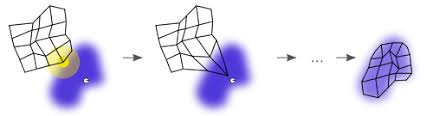
\includegraphics[scale=0.5]{som-learning}
    \caption{A SOM mapping the training data to a two dimensional grid.}
    \label{fig:som-learning}
\end{figure}
 
    \section{Previous Work}

Using machine learning for condition monitoring is not new.
There are typically three approaches:
\begin{enumerate}
	\item Supervised algorithms using sensor data and maintenance data.
    \item Unsupervised algorithms using only sensor data.
    \item Semi-supervised algorithms using only \textit{healthy} sensor data.
\end{enumerate}

% supervised
Supervised methods require labelled data.
Labelling is the process of associating an output with a set of variable values at a certain point in time.
For example, if there is knowledge to when the failures occurred and there are sufficient failures, the data can be labelled as healthy or not.
Unfortunately, there is just not enough failure data in practice to make this feasible.
Failure data can be estimated and artificially generated but even then the algorithms are limited to a binary outputs \cite{Sotiris2010AnomalyDT}.

Using $k$-nearest neighbours (kNN) to estimate asset condition directly is difficult due to noise, and requires domain specific knowledge to choose appropriate variables.
One paper improves on kNN methods for detecting the levels of severity for cracks in gears \cite{lei2009gear}.
The disadvantage in these approaches is that it requires significant data in a variety of conditions, and it uses classification to identify a severity level instead of a numerical value.

Researchers in \cite{opt} train an autoencoder on healthy imaging data to get a feature representation in a smaller number of dimensions.
Utilizing the Support Vector Machine (SVM), they learn a decision boundary to identify anomalies.
This approach is interesting for high dimensional data but focuses on point anomalies, where as we are interested in projecting asset health over time.

% self organized maps
SOMs have been used in condition maintenance as visualization tools for aircraft engines and ball bearings \cite{come2010aircraft}.
By mapping the input data to a two dimensional grid researchers can identify failures trends.
%Training a SOM on healthy asset data, researchers were able to output a health indication in an interpretable way but still lacked a quantifiable measure \cite{5524339}.
Alternatively, Huang et al. were able to use the minimum quantization error (Eq. \ref{eq:q}) between a test point and the closest neuron of the SOM as the health indicator for ball bearings \cite{som-1}.
% Math equation/formula
\begin{equation}\label{eq:q}
	Q = \min_{k} \Vert D-B_k \Vert
\end{equation}
Where $Q$ is the minimum quantization error, $D$ is a test set observation, and $B_k$ is the weight vector of the $k^{th}$ closest neuron of the SOM.
But, using quantization error can be improved as it is sensitive to noise.
Researchers Tian et al. use a SOM and a $k$-nearest neighbours algorithm in combination with the Euclidean distance between the test data and the healthy data to develop a more robust health score \cite{Tian2014AnomalyDU}.

   
    \section{Implementation}
\subsection{Overview}
The project will solve PdM hurdles for operators in modernized workplaces by providing an accurate estimate of asset health.
The proposed method is to replicate the results achieved by other papers using SOMs for condition monitoring. 
Specifically, to train a SOM and get a health score by calculating how much a test data point deviates from normal operation.
The higher the health score, the lower the operating condition of the asset.
%Various SOM implementations will be examined, such as the \href{https://pypi.org/project/kohonen/}{Kohonen 1.1.2 Python package} (documentation for this package is sparse).
%If these do not provide enough customization then a SOM will be self-coded using Tensorflow.
%Customization may be required to allow the comparison of various distance metrics to get a health score.
As discussed, this has been done before but is rarely seen in industry today and the use of these algorithms on real and significant data is challenging and relevant.
For example, the data will be provided in hourly chunks throughout the year (instead of one continuous data set).
Furthermore, feature engineering techniques are be explored to improve performance, use-ability and interpretability.
%Decision boundaries will be learned as a final step (if we have enough failure data) to organize failures into different classes and severity levels.
\begin{figure}[!h]
    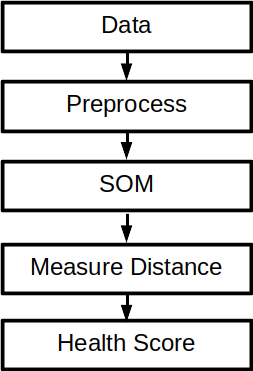
\includegraphics[width=3cm]{steps}
    \centering
    \label{fig:steps}
    \caption{Implementation steps from Data.}
\end{figure}

\subsection{Feature Engineering}
There are vibration signals used for the following: the interior bearing of the fan, 
the outer bearing of the fan, 
the interior bearing of the motor, and
the outer bearing of the motor (Figure \ref{fig:raw-signals}). 
The mean, standard deviation, skewness, kurtosis, and peak to peak were calculated every five minutes for each of the variables.
These five time domain features are commonly used to describe a signal \cite{Tian2014AnomalyDU}.
Additionally, the correlation between the signal and the other three was added as it increased the performance of the SOM.

\begin{figure}[!h]
    \centering
    \begin{subfigure}{6cm}
        \centering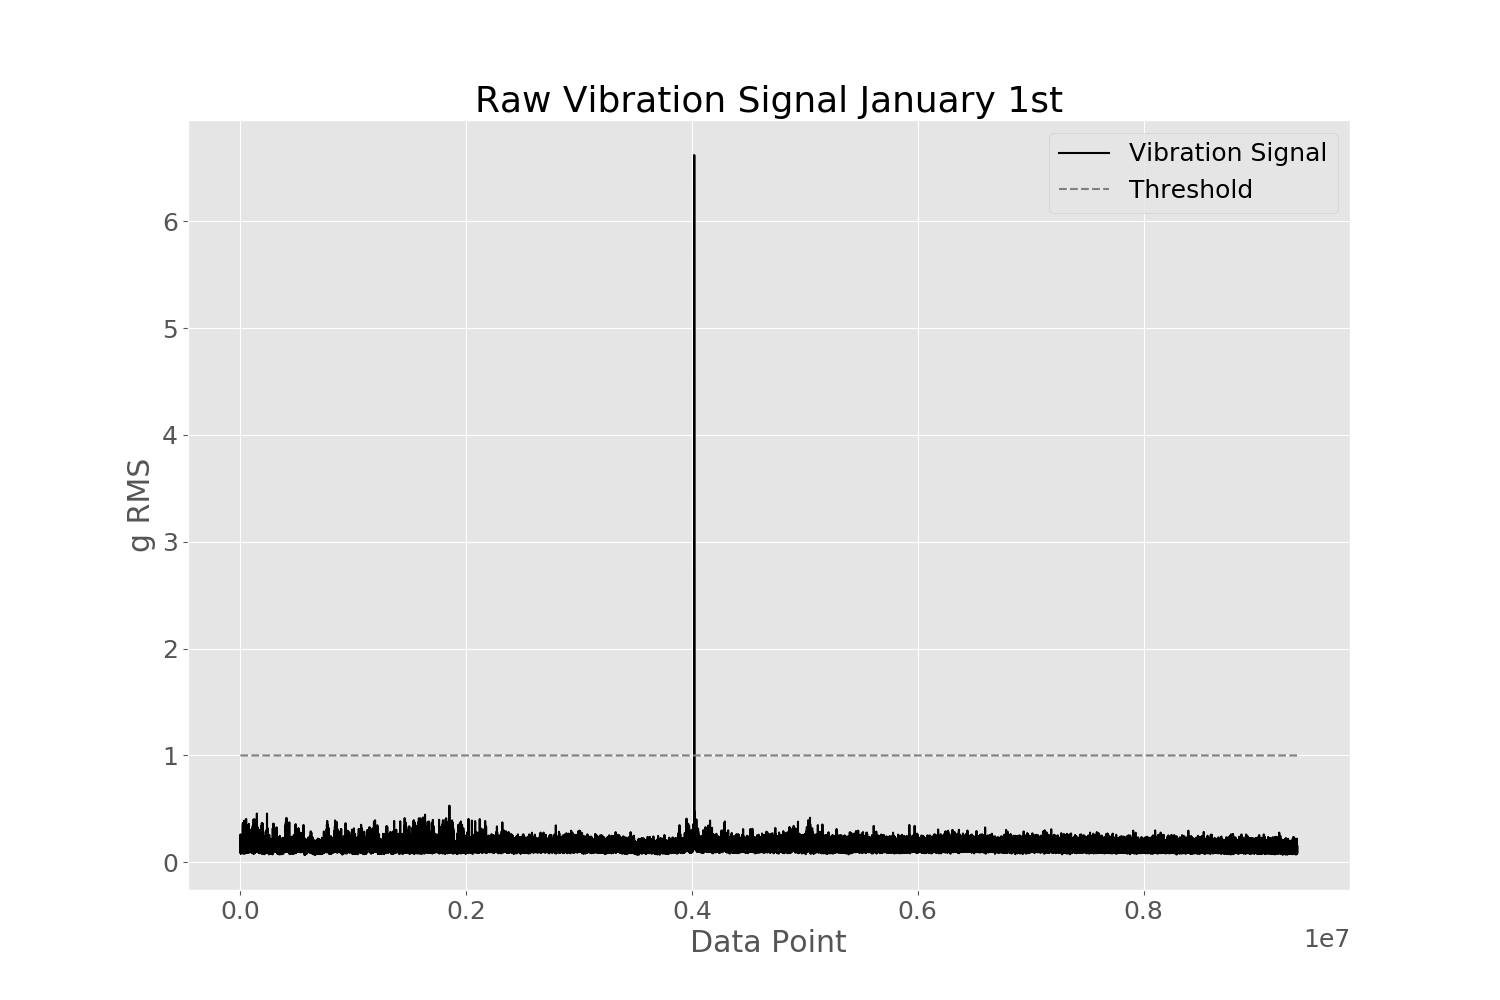
\includegraphics[trim={300 50 50 50}, width=\linewidth]{raw-jan1}
    \end{subfigure}%
    \begin{subfigure}{6cm}
        \centering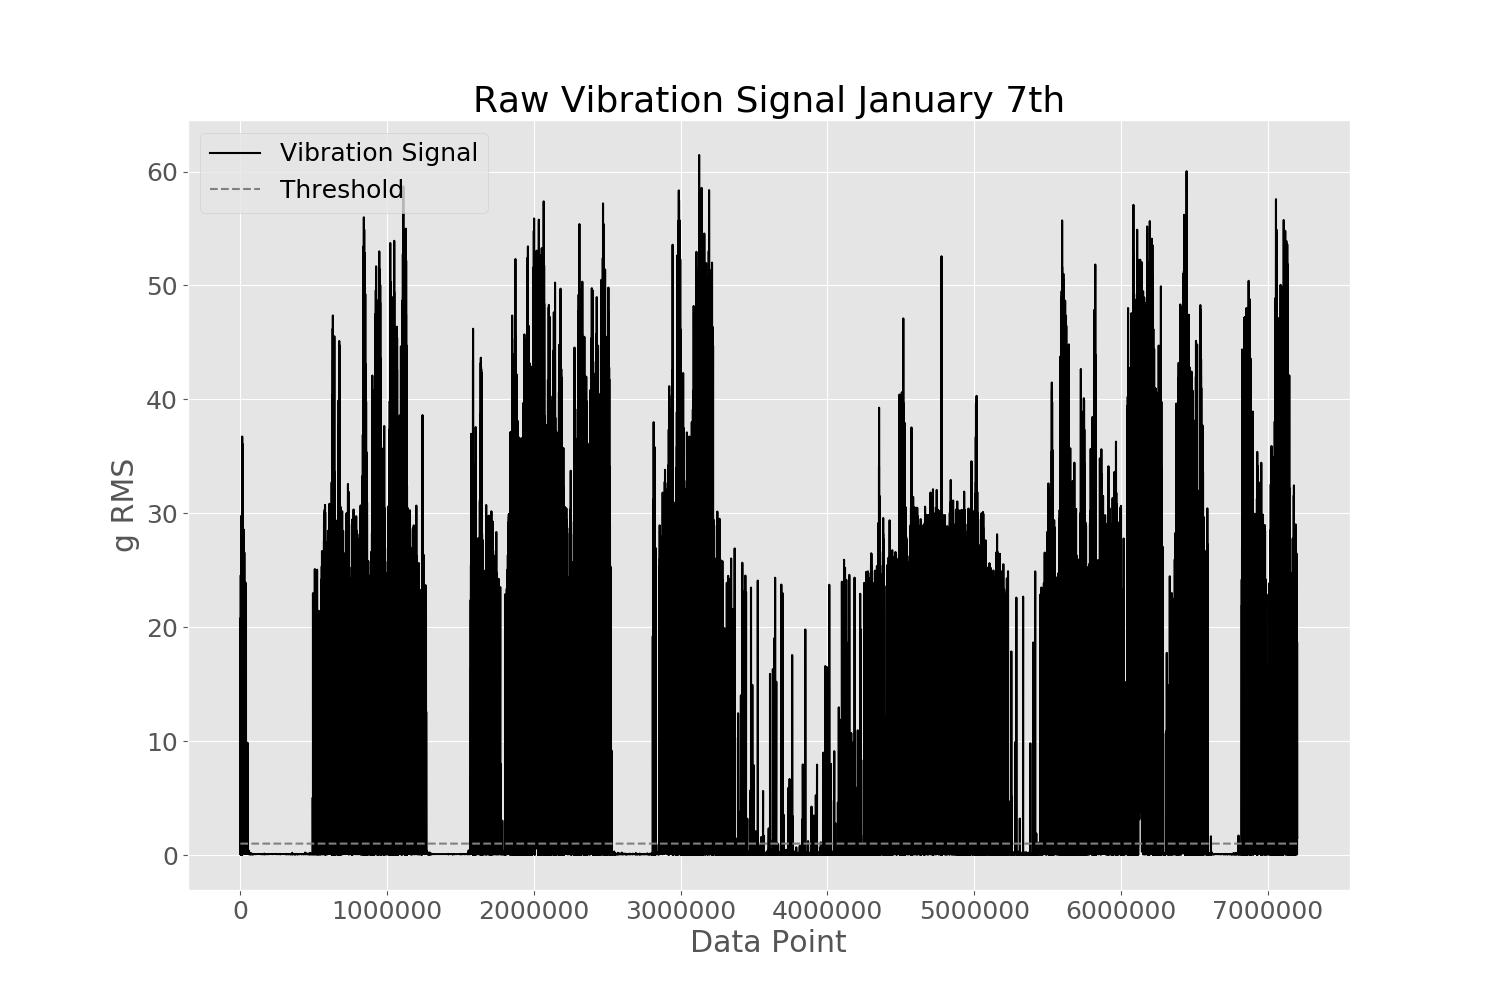
\includegraphics[trim={50 50 300 50}, width=\linewidth]{raw-jan7}
    \end{subfigure}\vspace{10pt}
 
    \begin{subfigure}{6cm}
        \centering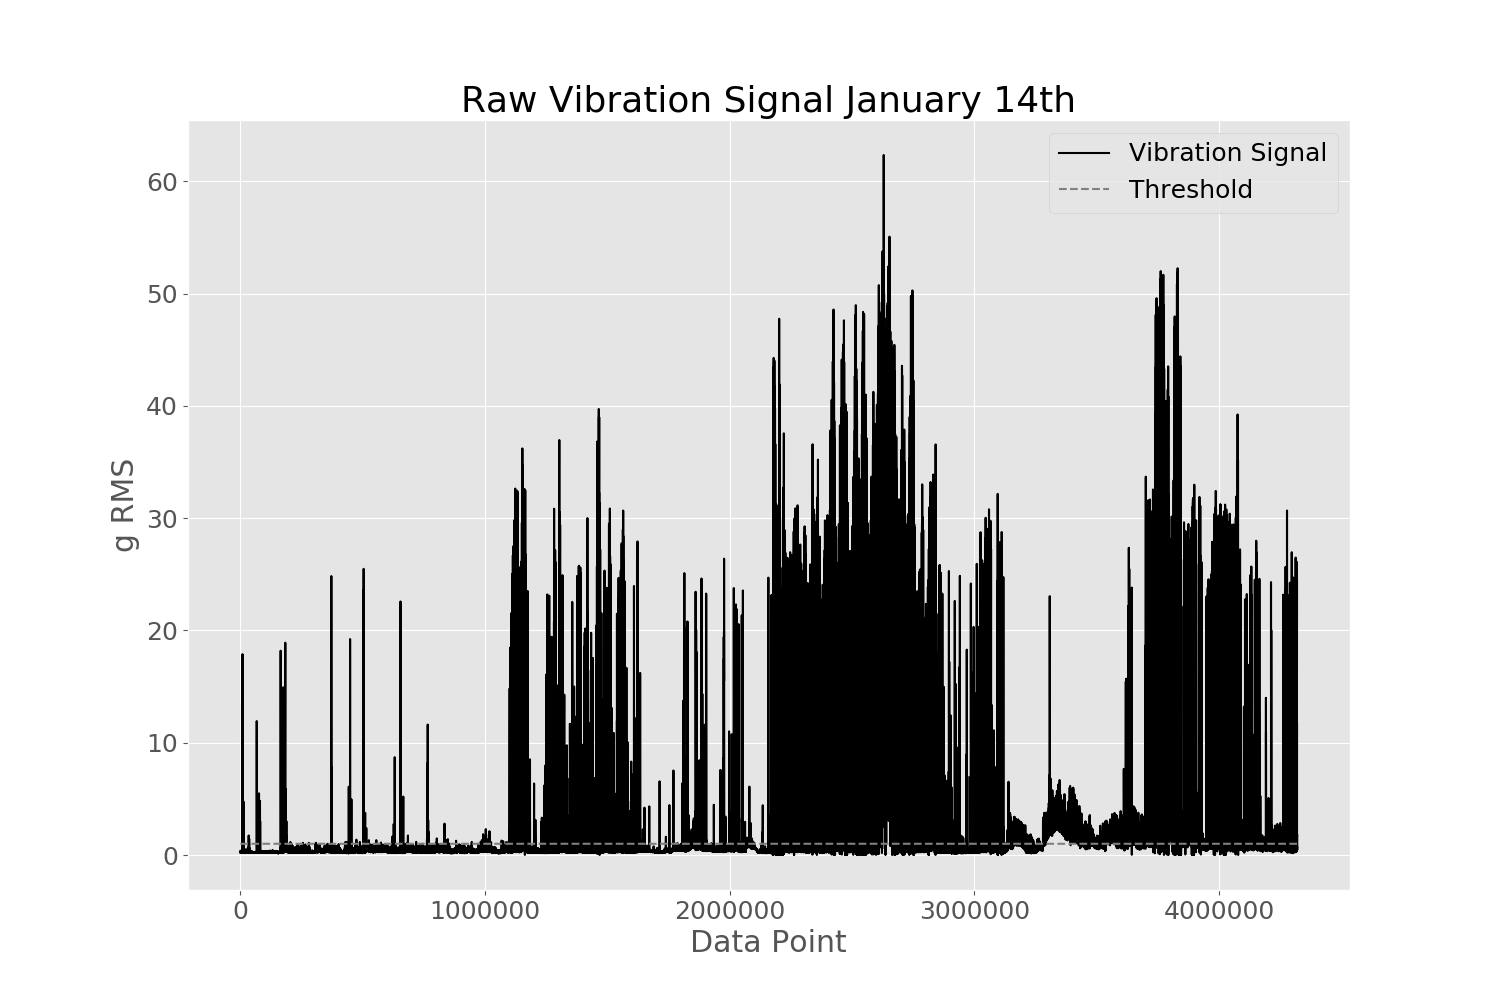
\includegraphics[trim={300 50 50 50}, width=\linewidth]{raw-jan14}
    \end{subfigure}%
    \begin{subfigure}{6cm}
        \centering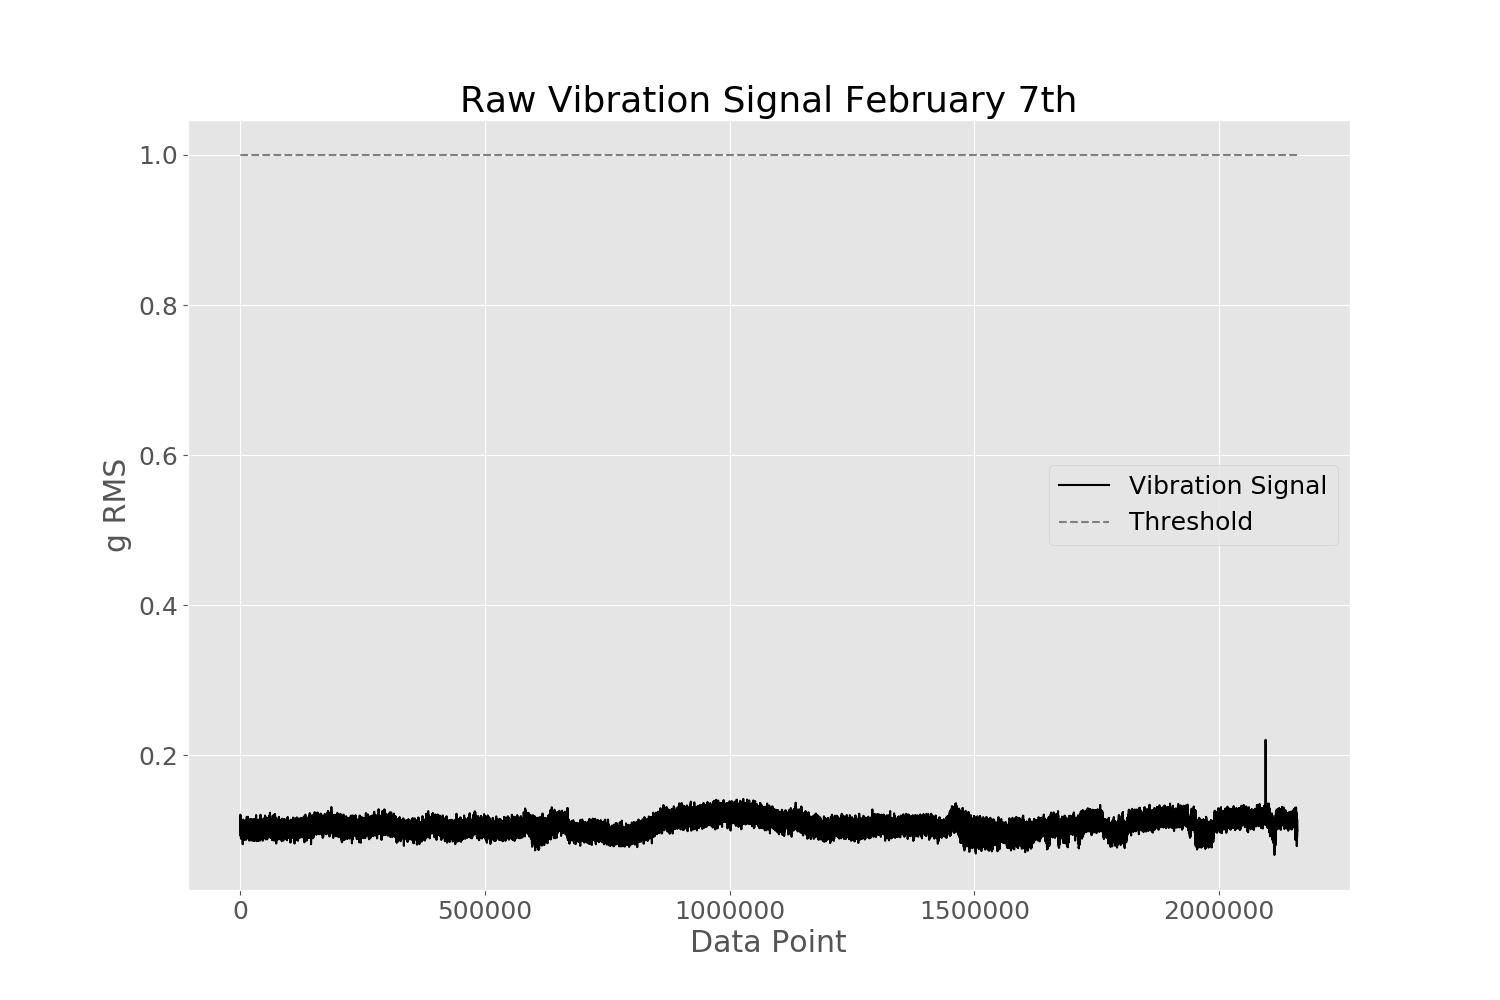
\includegraphics[trim={50 50 300 50}, width=\linewidth]{raw-feb7}
    \end{subfigure}
    \caption{Raw vibration signals.}
    \label{fig:raw-signals}
\end{figure}

    \newpage

    \nocite{*}
    
    \bibliographystyle{unsrtnat}
    \bibliography{sections/bibliography}

    \newpage
    \section*{Appendix}

% variable Table
\begin{table}[!h]
    \begin{tabular}{ll}
    \textbf{Variable Name}                   & \textbf{Description }                                   \\ \hline
    F1S F1SFIBV Overall (g RMS pk)           & Furnace 1 south fan inboard bearing vibration        \\
    F1S F1SFOBV Overall (g RMS pk)           & Furnace 1 south fan outboard bearing vibration       \\
    F1S F1SSMIBV Overall (g RMS pk)          & Furnace 1 south fan motor inboard bearing vibration  \\
    F1S F1SMOBV Overall (g RMS pk)           & Furnace 1 south motor outboard bearing vibration     \\
    F1S F1NFIBV Overall (g RMS pk)           & Furnace 1 north fan inboard bearing vibration        \\
    F1S F1NFOBV Overall (g RMS pk)           & Furnace 1 north fan outboard bearing vibration       \\
    F1S F1NMIBV Overall (g RMS pk)           & Furnace 1 north fan motor inboard bearing vibration  \\
    F1S F1NMOBV Overall (g RMS pk)           & Furnace 1 north fan motor outboard bearing vibration \\
    F1S North Fan Impellor side bearing temp & Furnace 1 north fan outboard bearing temp            \\
    F1S North Fan Motor side bearing temp    & Furnace 1 north fan inboard bearing temp             \\
    F1S South Fan Impellor side bearing temp & Furnace 1 south fan outboard bearing temp            \\
    F1S South Fan Motor side bearing temp    & Furnace 1 south fan inboard bearing temp            
    \end{tabular}
    \label{tbl:var}
    \caption{Variable names and descriptions provided by subject matter expert at ArclorMittal Dofasco plant.}
\end{table}

    
    \end{document}